\documentclass[border=4pt]{standalone}
\usepackage{tikz}
\usetikzlibrary{shapes.geometric,arrows.meta,positioning}
\definecolor{boxblue}{RGB}{225,238,252}
\definecolor{boxgreen}{RGB}{225,247,231}
\definecolor{boxorange}{RGB}{253,236,216}
\definecolor{boxgray}{RGB}{237,237,237}
\begin{document}
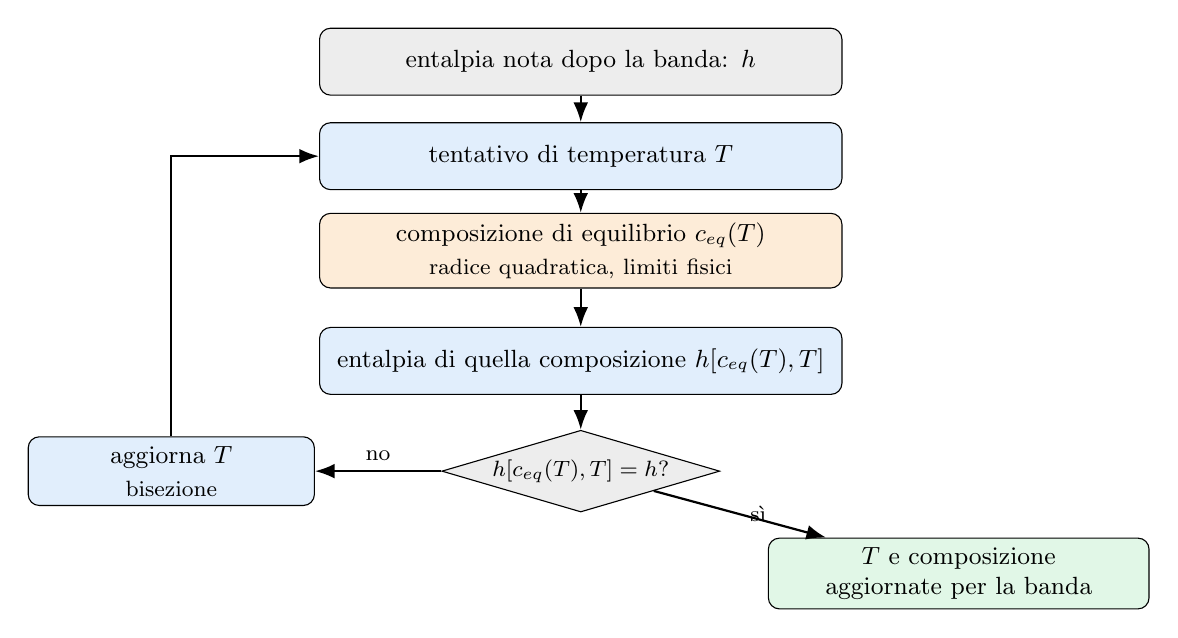
\begin{tikzpicture}[
  box/.style={draw, rectangle, rounded corners, minimum height=0.85cm, text width=6.4cm, align=center, font=\small},
  dec/.style={draw, diamond, aspect=3.4, align=center, font=\footnotesize, inner sep=1pt},
  arr/.style={-{Latex[length=2.5mm]}, thick}
]
\node[box, fill=boxgray] (h) at (0,0) {entalpia nota dopo la banda: $h$};
\node[box, fill=boxblue] (t) at (0,-1.2) {tentativo di temperatura $T$};
\node[box, fill=boxorange] (c) at (0,-2.4) {composizione di equilibrio $c_{eq}(T)$\\[1pt]\footnotesize radice quadratica, limiti fisici};
\node[box, fill=boxblue] (hh) at (0,-3.8) {entalpia di quella composizione $h[c_{eq}(T),T]$};
\node[dec, fill=boxgray] (d) at (0,-5.2) {$h[c_{eq}(T),T] = h$?};
\node[box, fill=boxblue, text width=3.4cm] (b) at (-5.2,-5.2) {aggiorna $T$\\[1pt]\footnotesize bisezione};
\node[box, fill=boxgreen, text width=4.6cm] (o) at (4.8,-6.5) {$T$ e composizione\\ aggiornate per la banda};
\draw[arr] (h) -- (t);
\draw[arr] (t) -- (c);
\draw[arr] (c) -- (hh);
\draw[arr] (hh) -- (d);
\draw[arr] (d) -- node[above,font=\footnotesize]{no} (b);
\draw[arr] (b) |- (t);
\draw[arr] (d) -- node[right,font=\footnotesize]{sì} (o);
\end{tikzpicture}
\end{document}
